\documentclass[../CourseManual.tex]{subfiles}

\begin{document}

The first algorithm that will be discussed is the formation algorithm. This algorithm is designed to have a system of agents converge to the same position. This is useful if the agents need to meet at a single point or surround a target.

\subsection{Formation Consensus Dynamics} \label{Formation Consensus Dynamics}
The formation algorithm is an averaging function that takes in agent positions and returns agent velocities. The continuous-time dynamics of the system can be described by the first order differential equation 

$$ \boldsymbol{\dot{q}} = - L \cdot \boldsymbol{q},$$

where $\boldsymbol{q}$ is an $n \times 2$  position vector containing the $(x, y)$ coordinate pairings for each of the $n$ agents in the system. In other words, the entry in the $i$-th row of the first column of $\boldsymbol{q}$ contains the $x$ coordinate of $i$-th agent. Similarly, the entry in the $i$-th row of the second column of $\boldsymbol{q}$ contains the $y$ coordinate of $i$-th agent. The Laplacian matrix, $L$, is a function of the adjacency matrix, $A$, and the degree matrix, $D$, and can be calculated by

\[ 
L = D -A.
\]
The adjacency matrix of the system is an $n \times n$ matrix given by
\[ 
A(i,j) = 
\begin{cases}
 1, & \text{ if agent $i$ receives communication from agent $j$,}\\
 0, & \text{ if agent $i$ does not receive communication from agent $j$.}
\end{cases}
\]

The degree matrix of the system is a diagonal $n \times n$ matrix given by
\[
D(i,i) = \sum_{j=1}^{n}{A(i,j)}.
\]

Hence, the Laplacian matrix for the system is an $n \times n$ matrix that has the property

\[
L \cdot
\begin{bmatrix}
\alpha \\
\alpha \\
\vdots \\
\alpha \\
\end{bmatrix}
=
\begin{bmatrix}
0 \\
0 \\
\vdots \\
0\\
\end{bmatrix}
\forall \alpha \in \mathbb{R}.
\]

In other words, the sum of each row is zero (and each column since the matrix is symmetric). This implies that $\boldsymbol{\dot{q}} = [0,0,...,0]^T$ if $q_i = q_j$ for all $i,j \in [1,n]$. In order to model the formation algorithm, the system must be discretized from a continuous system. In the discrete time domain, the system updates the position of each agent using
\[
\boldsymbol{q}(t + \Delta t) = \boldsymbol{q}(t) - L \cdot \boldsymbol{q}(t) \cdot \Delta t,
\]
where $\Delta t$ is a fixed time increment. In addition, the adjacency matrix for your system will most likely not be the same throughout the simulation. Entries in your adjacency matrix will be dependent on your system's current state and design constraints.

\subsubsection{Introducing Offsets} \label{Introducing Offsets}
Offsets are differences between an agent's final position and the consensus position of the system. Instead of agents moving to an average in a decentralized way, setting an offset allows you to set where individual agents will move (with the network average as the origin). For instance, if the consensus position of the system is (1,2) and an agent has an $x$ offset of 1 and a $y$ offset of -2, the agent will converge to the point (2,0). The only change in the system dynamics when offsets are introduced is within the position update step
\[
\boldsymbol{q}(t+\Delta t) = \boldsymbol{q}(t) - L \cdot [\boldsymbol{q} - \boldsymbol{g}] \cdot \Delta t,
\]
where $\boldsymbol{g}$ is an offset vector of dimension $n \times 2$ containing the $x$ and $y$ offsets for all agents.

\subsubsection{Introducing Delays} \label{Introducing Delays}
Delays are time steps where agents are idle before responding to changes in the system and moving to a new position. If an agent has an infinite delay, it is referred to as a ``stubborn" agent and is described by $\boldsymbol{\dot{q}} = 0, \forall t \in \mathbb{R}_{\geq0}$. Otherwise, agent $i$ will update $\tau_i \in \mathbb{R}_{\geq0}$ times-steps late when responding to a movement signal. With time delays, the position update equation is now
\[
\boldsymbol{q}(t+\Delta t) =
\begin{bmatrix}
q_1(t-\tau_1)\\
q_2(t-\tau_2)\\
\vdots \\
q_N(t-\tau_N)\\
\end{bmatrix}
- L \cdot [\boldsymbol{q}(t) - \boldsymbol{g}] \cdot \Delta t.
\]

\subsection{Simulation App} \label{Simulation App: Formation}
The app provided uses the consensus dynamics to update each agent's location for every iteration of the simulation. The critical components of the app's functionality have been placed in external functions, which you will develop over the course of the project. The functions that you will be responsible for are discussed in detail in \hyperref[MATLAB Functions: Formation]{Section \ref{MATLAB Functions: Formation}}. \\

Upon simulation completion, the app will create an excel file named \textit{agentData.xlsx} containing the positions, energy, and distance to mean for all agents, throughout the duration of the simulation. This data should be used to conduct further analysis to improve or validate your design.

%app picture goes before the descriptions
\begin{figure}[H]
    \centering
    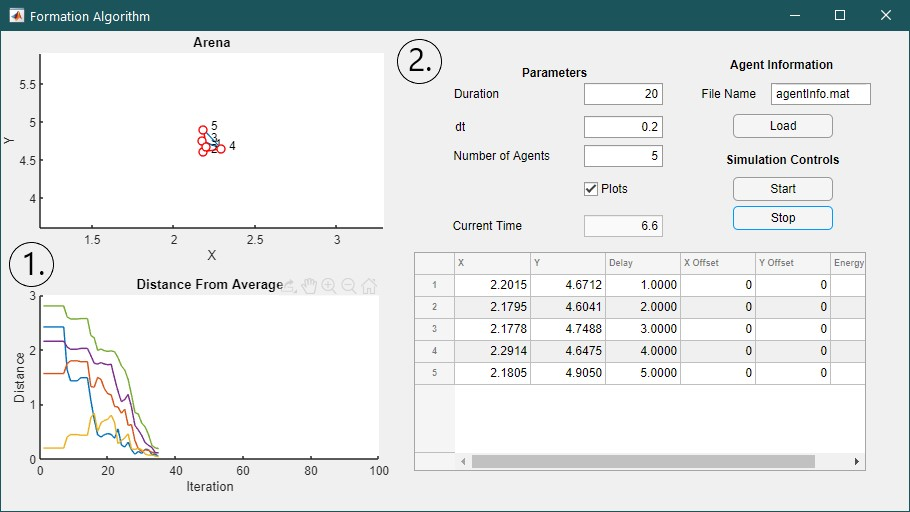
\includegraphics[width=350pt]{media/Formation.jpg}
    \caption{Screen capture of FormationApp.mlapp with default settings}
    \label{fig: formation app}
\end{figure}

\subsubsection{Plots}
Area 1 of Figure \ref{fig: formation app} displays the plots section of the Formation app. This section contains two separate plots, the \textbf{Arena} plot and the \textbf{Distance From Average} plot. \\

The plot in the top left portion of the app window is the \textbf{Arena} plot. The position of each agent is displayed as a dot with a numerical label on the plot. The lines connecting agents represent the communication graph as determined by the adjacency matrix. This plot is updated every iteration of the simulation to visualize the movement of the agents throughout the simulation. \\

The second plot in the app window is the \textbf{Distance From Average} plot. Upon initiation of the simulation, the consensus (average) position is calculated. Then, the distance between each agent and the consensus position is calculated and plotted for every iteration. The resultant plot effectively tracks agents as they converge to the consensus position. The independent axis displays simulated time whilst the dependent axis plots distance between agent and consensus position.
 
\subsubsection{User Controls} \label{User Controls: Formation}
Area 2 of Figure \ref{fig: formation app} displays the user controls section of the Formation app. This section is divided into three sub-sections: the \textbf{Parameters} sub-section, the \textbf{Agent Information} sub-section, and the \textbf{Simulation Controls} sub-section. \\

The \textbf{Parameters} sub-section  is where you can alter the simulation parameters which affect the number of agents and the duration. The number of agents to be used in the simulation can be adjusted by the user by changing the value in the \textbf{Number of Agents} edit field. If plotting is enabled, the agent data table will be updated every iteration to reflect any changes in each agents' properties. The \textbf{Duration} edit field allows the user to adjust the simulation duration in arbitrary units of time. The \textbf{Current Time} edit field is non-editable and displays the current time while the simulation is running. The value of $\Delta t$ in the position update equation in \hyperref[Formation Consensus Dynamics]{Section \ref{Formation Consensus Dynamics}} can be modified via the \textbf{dt} edit field. The \textbf{Plots} checkbox, when enabled, will update the \textbf{Arena} plot, the \textbf{Distance From Average} plot, and the \textbf{Agent Information} table on every iteration. Disabling \textbf{Plots} will greatly increase the speed of your simulation. This is useful if you need to simulate for more than a few hundred iterations. The table in the app contains five columns: the current \textit{x} and \textit{y} positions; \textit{delay}; \textit{x offset}; \textit{y offset}; and \textit{energy}. This data can be edited directly or loaded from a file created in the Matrix Editor. See \hyperref[Matrix Editor: Formation]{Section \ref{Matrix Editor: Formation}} for details.\\

The \textbf{Simulation Controls} sub-section contains the \textbf{Start} button which begins the simulation and the \textbf{Stop} button which stops the simulation before completion. \\

The \textbf{Agent Information} sub-section allows you to load in the initial conditions for the agents by specifying a .mat file name under the \textbf{Agent Information} heading and pressing \textbf{Load}, avoiding the need to manually re-enter data. \\

\subsubsection{Matrix Editor} \label{Matrix Editor: Formation}

Using the \textbf{Matrix Editor Formation} app, you are able to create files for initial agent data. To do so, first enter the number of agents in the \textbf{Number of Agents} edit field. Next, edit the values in the table as you see fit. When complete, specify a filename including the \textit{.mat} extension. Remember to enter this filename and press the \textbf{Load} button in the simulation app to load the data you have entered.

\begin{figure}[H]
    \centering
    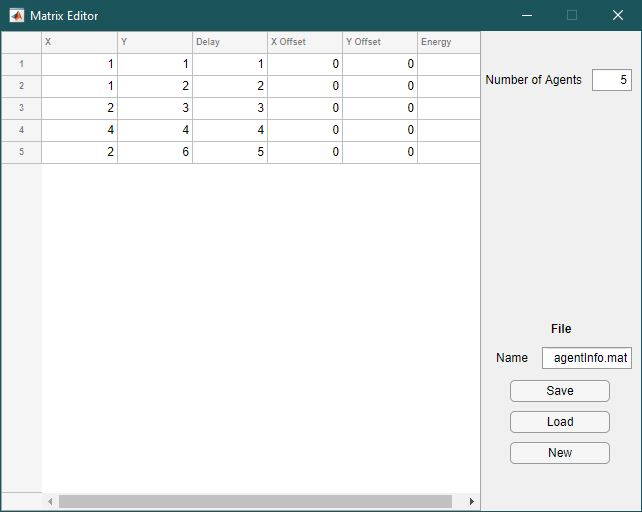
\includegraphics[width=350pt]{media/MatrixEditorFormation.JPG}
    \caption{Screen capture of MatrixEditorFormation.mlapp with default settings}
    \label{fig: matrix editor formation}
\end{figure}

\subsubsection{Parameters and Variables}

\renewcommand{\labelenumi}{\roman{enumi}}
\begin{enumerate}

    \item Number of Agents $(numAgents)$: Total number of agents $(N)$ used in simulation.
  
    \item Agent Position $(agentPosition)$: An $N \times 2$ matrix with the x-position of the $i^{th}$-agent in the first column of row $i$, and the y-positions in the second column, as below:
  
    $$Agent Positions = 
    \begin{bmatrix}
    q^{1}_{x} \hspace{0.5cm} q^{1}_{y}\\
    q^{2}_{x} \hspace{0.5cm} q^{2}_{y}\\
    \vdots \hspace{0.5cm} \vdots \\
    q^{N}_{x} \hspace{0.5cm} q^{N}_{y}\\
    \end{bmatrix}$$
    
    \item Adjacency Matrix $(A)$: The $N \times N$ adjacency matrix:
    
    $$ 
    A(i,j) = 
    \begin{cases}
     1, & \text{ if agent $i$ receives communication from agent $j$,}\\
     0, & \text{ if agent $i$ does not receive communication from agent $j$.}
    \end{cases}
    $$
    
    \item Degree Matrix $(D)$: The $N \times N$ degree matrix:
    
    \[
    D(i,i) = \sum_{j=1}^{n}{A(i,j)}.
    \]
    
    \item Laplacian Matrix $(L)$: The $N \times N$ Laplacian matrix:
    
    $$L = D - A$$
    
    \item Duration $(duration)$: Total duration the simulation will run for.
    
    \item $\Delta t$ $(dt)$: Amount of time simulated in each iteration.
    
    \item Current Time $(time)$: Current (simulated) time.
    
    \item Positional Offset: The $x$ and $y$ positional offsets are saved within column 4 and 5 of the $N \times 6$ vector $agentData$. The positional offsets determine where agents will converge to with respect to the network average. Mathematically, this alters the position update equation as seen in \hyperref[Introducing Offsets]{Section \ref{Introducing Offsets}} to be the equation
    
    $$
    \boldsymbol{q}(t+\Delta t) = \boldsymbol{q}(t) - L \cdot [\boldsymbol{q} - \boldsymbol{g}] \cdot \Delta t,
    $$
    where $\boldsymbol{g}$ is an offset vector of dimension $n \times 2$ containing the $x$ and $y$ offsets for all agents.
    
    \item Time Delay: The time delays are saved within column 3 of the $N \times 6$ vector $agentData$. The  time delays determine the delay in an agent's reaction time when updating it's position. Mathematically, this alters the position update equation as seen in \hyperref[Introducing Delays]{Section \ref{Introducing Delays}} to be the equation

    $$
    \boldsymbol{q}(t+\Delta t) =
    \begin{bmatrix}
    q_1(t-\tau_1)\\
    q_2(t-\tau_2)\\
    \vdots \\
    q_N(t-\tau_N)\\
    \end{bmatrix}
    - L \cdot [\boldsymbol{q}(t) - \boldsymbol{g}] \cdot \Delta t.
    $$
    
    \item Energy: The energy metric is saved within column 6 of the $N \times 6$ vector $agentData$. You must determine the units of the energy that you wish to use and how you want to represent this in the energy array. The energy will decrease after every iteration by some parameter (you may choose how to represent this).
    
    \item Agent Data $(agentData)$: The agent data matrix is the $N \times 6$ matrix which contains the $x$ positions of the agents in the $1^{st}$ column, the $y$ positions of the agents in the $2^{nd}$ column, the delay values in the $3^{rd}$ column, the $x$ offset values in the $4^{th}$ column, the $y$ offset values in the $5^{th}$ column, and the energy values in the $6^{th}$ column.
    
\end{enumerate}

\subsubsection{MATLAB Functions} \label{MATLAB Functions: Formation}
    The following MATLAB functions that you will need to write in order for the simulation app to function are described below. The order that functions are listed is the order that you will be creating them during the project.\\

    \textbf{calcA.m} --  calcA.m is used to calculate the adjacency matrix based on the agent states and any relevant design constraints. The calcA function will take as input $agentPosition$ and will output $A$. $A$'s calculation will be determined by you in Week 2. \\

    \textbf{calcL.m} -- calcL.m is used to calculate the Laplacian matrix for the current iteration of the simulation using the adjacency matrix. The CalcL function takes as input $A$ and outputs $L$. $L$ is calculated as seen in \hyperref[Formation Consensus Dynamics]{Section \ref{Formation Consensus Dynamics}} with the equation 

    $$L = D - A$$

    \textbf{moveAgents.m} -- moveAgents.m is used to update the position of each agent using the consensus dynamics formula in \hyperref[Formation Consensus Dynamics]{Section \ref{Formation Consensus Dynamics}}. The moveAgents function takes inputs $agentData$, $L$, $time$, and $dt$, and outputs $agentData$. The positional data in $agentData$ is updated as seen in \hyperref[Formation Consensus Dynamics]{Section \ref{Formation Consensus Dynamics}} with the equation 

    $$
    \boldsymbol{q}(t+\Delta t) =
    \begin{bmatrix}
    q_1(t-\tau_1)\\
    q_2(t-\tau_2)\\
    \vdots \\
    q_N(t-\tau_N)\\
    \end{bmatrix}
    - L \cdot [\boldsymbol{q}(t) - \boldsymbol{g}] \cdot \Delta t.
    $$

    Furthermore, in week 4 you will be tasked to model and introduce a cost function involving the energy parameter into the moveAgents function.

\subsection{Example: Formation} \label{Example: Formation}
    This section provides a sample P2 project using the formation algorithm. This example is broken up into what is to be completed each week of the project to provide a reference to what will be expected in your projects. You can not use this application area for your project.

    \subsubsection{Week 1} \label{Week 1: Formation}
        \textbf{Area of Application}\\
        The application area that has been selected involves using a number of submersible vehicles to conduct research on coral bleaching in a shallow sea. There are a number of submersibles sampling coral over an area of several squared kilometers. The submersibles take samples until their on-board storage containers are full. Instead of wasting time and resources by having each agent return to shore to deliver its samples, a ship is to be sent out to the first agent’s location. The other agents are to meet the ship at the first agent's location. However, communication underwater is difficult and costly, which restricts the communication abilities between agents.\\

        \textbf{Algorithm Selection}\\
        With a potential area of application selected, each of the possible group dynamics algorithms are examined in more detail. Based on the application area's requirement that the agents converge to a single location, it was determined that the formation algorithm was the most suitable choice for the project.\\

        \textbf{Pitch Presentation}\\
        With the area of application selected, a brief pitch presentation of the application area is created. This presentation provides a high-level overview of the area of application and how a group-formation algorithm could be applied to model the design solution. 

    \subsubsection{Week 2} \label{Week 2: Formation}
        \textbf{Proposal Report}\\
        With the application area and formation algorithm selected, the proposal report can now be written. This report includes all the standard items listed on the rubric, such as an executive summary, introduction with background information, discussion, project plan, etc. The problem definition specifies that a performance analysis needs to be conducted on several models of submersible robots to determine the efficacy and economic viability of each system model. The main stakeholders are identified and include: the research group, the submersible vehicle company, state/federal governments, and more. Design metrics include time to convergence, travel range, redundancy in communication (i.e. fail-safe system), cargo capacity, initial cost(s), operational cost(s), maintenance cost(s), and robot lifespan. \\

% REV 2 SUBMERSIBLE TYPES: Two potential submersible robots have been selected for this project. The first is the Submersible Robot 1 (SR1) and the second is the Submersible Robot 2 (SR2). The research group has specified the need for a cargo capacity of at least 10 units per mission. Examination of the technical documentation for the SR1 and SR2 reveals they have a cargo capacity of 1.25 and 2 units, respectively. This means that, based on the cargo capacity requirements, 8 SR1 submersibles or 5 SR2 submersibles would be required at minimum. \\

\textbf{Adjacency Matrix}\\
% REV 1 A MATRIX: A system comprised of 8 SR1s has an 8-by-8 adjacency matrix. The SR1 technical documentation specifies that communication is unidirectional, i.e. agents can only communicate with one other agent in the system. Thus, a linear communication chain is required. Given that the first agent is at the ship's location, the other resulting adjacency matrix for the system will be of the following form:

Various communication methods between agents will be developed and then tested using the simulation. Each method will be defined using a number of design parameters. These parameters include the number of agents, the number of possible communication pairings for each agent, the distance between a pair of communicating agents and the radius of communication for each agent. These exact values are not defined at this point and will be determined through simulation testing and evaluation against a set of design metrics (these metrics will be defined in Week's 4 and 5).\\

The first potential communication method has the agents form a communication chain such that each agent can only communicate with the agent before itself. The exception to this chain will be with agent 1, which will not have a communication partner. This is done so that it does not move from its starting location, thus acting as the point of convergence for the other agents.\\

Another method is having each agent be in communication with the agent before and after itself. Like the first method, the first agent will not have any communication partners to ensure all agents converge to its starting position. For the last agent in this communication chain, it will only have one communication partner, the agent before itself.\\

For both methods, the strength of communication between agent $i$ and its communication partner is determined using
\[
A(i,i-1) = 
\begin{cases}
 \frac{(d_{(i,i-1)}-r_c)^2}{r_c^2} , & d \leq r_c,\\
 0, & \text{otherwise,}
\end{cases}
\]
for agent $i-1$, the agent before itself, and 
\[
A(i,i+1) = 
\begin{cases}
 \frac{(d_{(i,i+1)}-r_c)^2}{r_c^2} , & d \leq r_c,\\
 0, & \text{otherwise,}
\end{cases}
\]

for agent $i+1$, the agent after itself. The radius of communication for the agent is denoted by $r_c$. For a communication pairing with the agent before itself, the distance between the two agents is denoted by $d_{(i,i-1)}$. Similarly, for a communication pairing with the agent after itself, the distance between the two agents is denoted by $d_{(i,i+1)}$. This method could be extended to include more communication partners for each agent up to all the agents being in communication with each other. \\

% REV 2 Adjacency Matrix
% For a system of 8 SR1s, the corresponding adjacency matrix would by an 8 by 8 matrix. The matrix would have a diagonal of ones indicating the submersibles can communicate with themselves. Each submersible would then be assigned to communicate with the agent after it (i.e. Agent 1 communicates with Agent 2 and Agent 2 communicates with Agent 3 and so on). The assignment of a unique communication partner ensures that all the submersibles return to the research vessel and do not stray off course. Agent 1 will not have a communication partner since all the agents are to converge to its current position to meet the research vessel. The SR1 submersibles have a defined radius of communication, $r_c$, of 3000 meters where the strength of the communications received dissipates over this radius to zero. Thus, the adjacency matrix for the system will be dependent on the current Euclidean distance, $d_{(i,i-1)}$, that the submersible is from its communication partner. The distance between communication partners, in meters, is calculated using the current position (current state) of each submersible.
%\[
%A(i,i-1) =
%\begin{cases}
%\frac{r_c^2}{(d_{(i,i-1)}-r_c)^2}, & d \leq 3000,\\
%0, & \text{otherwise.}
%\end{cases}
%\]

%Note that this adjacency matrix will be asymmetric since the communication channels are unidirectional. Also note that agent 8 will not be sending data to any agent, and agent 1 will not receiving data from any agent. The isolation of agent 1 ensures that it will not move, as specified previously.\\

%A system of 5 SR2s has a 5-by-5 adjacency matrix. Technical documentation for the SR2 specifies that communication is bidirectional in addition to being able to communicate with itself. This means that each agent can communicate with the agent before and after itself. For example, Agent 2 will be able to receive communications from Agents 1 and 3. The radius of communication, $r_c$ for each SR2 submersible is 2000 meters. Similar to the SR1 submersibles, the strength of communications received decreases over this radius to zero. Thus, this adjacency matrix will also be dependent on the current Euclidean distance between its communication partners which is calculated using the current positions (current state) of each agent. The strength of communication is determined using
%\[
%A(i,i-1) = 
%\begin{cases}
% \frac{r_c^2}{(d_{(i,i-1)}-r_c)^2} , & d \leq 2000,\\
% 0, & \text{otherwise,}
%\end{cases}
%\]
%for agent $i-1$, and 
%\[
%A(i,i+1) = 
%\begin{cases}
%\frac{r_c^2}{(d_{(i,i+1)}-r_c)^2} , & d \leq 2000,\\
% 0, & \text{otherwise,}
%\end{cases}
%\]

% for agent $i+1$. For Agent 1, its communication capabilities are modified such that it is only in communication with itself. This step is taken to ensure that agent 1 remains stationary so that all the agents converge to its position, which is also where the research vessel is. The last agent in the system, Agent 5 only has communication defined with Agent 4 since no Agent 6 exists.

\subsubsection{Week 3} \label{Week 3: Formation}
\textbf{MATLAB Coding}\\
The \textit{calcA.m} function is used to calculate the adjacency matrix for the system given its current state and design constraints. The resulting adjacency matrix is then used in the \textit{calcL.m} function to calculate the resulting Laplacian Matrix.\\

\textbf{Design Process} \\
Continue researching parameters that will be used to evaluate the final design. These metrics could include the maximum area of coverage by all the robots in the system, various performance specifications of the robots, the time to convergence and more. The parameters that will be evaluated using the simulation should also be noted. A method of scoring potential design solutions using the defined metrics should also be developed.\\ 

Begin research for the Triple Bottom Line (TBL) analysis of the project. This analysis focuses on the  social, economic and environmental impacts that the final design solution will have. This research could include; the financial impact on the research group in purchasing the final design solution,  the environmental impact of the submersible robots and many more. Determining how your design will influence these factors is important to keep in mind. Some areas may be important enough to include as a metric for design evaluation! \\

\textbf{Reports}\\
Complete the first progress report as outlined in the report template. This report is meant to highlight the items you have accomplished to date. The next steps for the project and areas of current or anticipated challenge should be noted with a plan on how these challenges will be overcome.

\subsubsection{Week 4} \label{Week 4: Formation}
\textbf{MATLAB Coding}\\
Translate the position update equation for the formation algorithm into code in \textit{moveAgents.m}. Within this function, we can model propagation delays in the communication system by setting
\[
\tau_i = 10\left( \frac{||\vec{q}_i(t) - \vec{q}_j(t)||}{1000} \right), 
\]
so that there is an extra 10 second delay for information sent from agent $j$ to agent $i$ for every 1000 meters between them. \\

% The time step, $\Delta t$, is determined by the frequency at which the SR1 and SR2 can transmit/receive data. Based on technical documentation, these values are 2 seconds and 5 seconds, respectively. The maximum cruising speeds for the SR1 and SR2 are 20km/h and 35km/h, respectively. \textit{moveAgents.m} checks for this to ensure that movement does not exceed maximum speeds. \\ 

\textbf{Design Process}\\
Energy levels within each submersible must be considered in the model as agents need to reach the ship before running out of fuel. The metric for an energy resource could be actual fuel energy, time, distance, etc., so long as the depletion of energy can be reasonably modelled and incorporated into the \textit{moveAgents.m} function. Conduct the necessary research to determine what the energy function will look like and the energy capacity available in each robot. The energy model for this example will take into account energy depletion due to work by drag and change in kinetic energy. Suppose after research that the SR1 has a full charge battery capacity of 150kJ, whereas the SR2 has 200kJ.\\

Decide on a decision making strategy for your final design. For example, if using an evaluation matrix, be sure to justify the design metrics and their weights through additional research.

\subsubsection{Week 5} \label{Week 5: Formation}
\textbf{MATLAB Coding}\\
Now comes time to integrate the energy function into \textit{moveAgents.m}. The remaining energy levels for each agent can be modelled by decreasing their energy based on the work done at each time step
\[
E_i(t+\Delta t) = E_i(t) - F_{d_i}(\vec{q}_i(t + \Delta t) - \vec{q}_i(t)) - P \Delta t,
\]
where $E_i$ is the energy remaining for the $i$th agent, $F_{d_i}$ is the force of drag on agent $i$, and $P$ is the constant power drawn per unit time while the robot is in use. This model assumes that the robot's speed is constant for each time step and that the only force acting against the robot's motion is drag. The drag for a body can be modelled using
\[
F_{d_i} = C_d\frac{1}{2}\rho V_i^2 A_i,
\]
where $C_d$ denotes the drag coefficient for the submersible \cite{NASA}. The submersible's velocity in $m/s$ and cross-sectional area perpendicular to direction of the submersible's travel are denoted by $V_i$ and $A_i$, respectively. The density of water is represented by $\rho$.\\
% REFERENCES FOR DRAG EQUATIONS
%       https://www.grc.nasa.gov/www/k-12/airplane/drageq.html

\textbf{Design Process}\\
The simulation should now be operational. Testing of the system with various sets of design parameters can be run with the simulation with the system's performance then being evaluated against the set design metrics. For example, testing for a radius of communication that provides a suitable level of performance to the system while remaining economically feasible could be now determined. Another example could be determining the optimum number of agents needed to provided the desired area of coverage. \\

\textbf{Reports}\\
Complete the second progress report as outlined in the report template. This report will be similar in structure to the first progress report.\\

Begin writing the final report detailing the Design Process, Design Solution and its evaluation against the Design Metrics, TBL Analysis and more. This report should include the revised sections from the proposal report based on the feedback given.

\subsubsection{Week 6} \label{Week 6: Formation}
\textbf{Final Design}\\
Review and finalize the evaluated design criteria for each design. Decide on a final proposed solution with justification. Create figures and tables for use in the final report and presentation. Complete the final report and presentation. Pay significant attention to documenting the design process, with justification of each step along the way (evaluation matrices, design rubrics, etc.)


\end{document}